%!TEX root = bachelor.tex
\chapter{Theoretische Grundlagen}
\label{ch:theory}

Links Koordinatensystem...

\section{Kegel}
\label{s:cone}

\begin{definition}[Kegel]
	kegel
	$S$ bezeichnet die Seitenhöhe und ist definiert durch $S = \sqrt{H^2 + R^2}$
	$S >= R$ Dreiecksungleichung
\end{definition}

In der weiteren Arbeit betrachten wir nur gerade Kreiskegel

\begin{figure}[!htb]
	\centering
	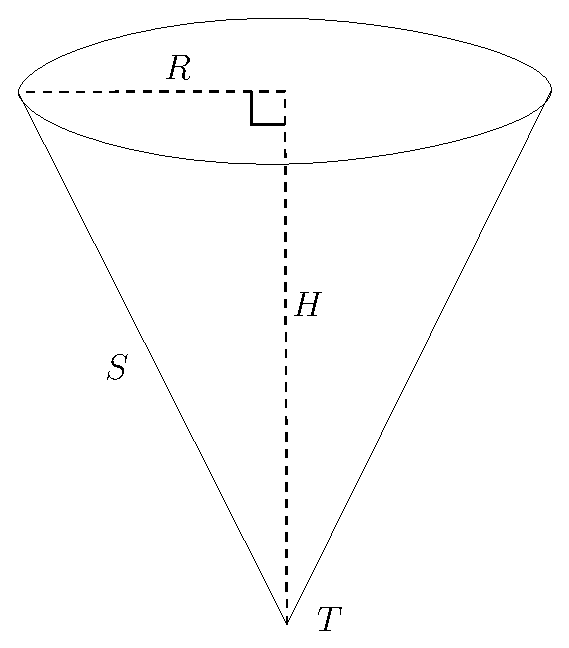
\includegraphics[scale=.5]{images/fullCone.eps}
	\caption{Gerader Kreiskegel}
	\label{fig:cone}
\end{figure}

Ein Kegel mit Spitze $T(0,0,0)$, Radius $R$ und Höhe $H$ kann parametrisch beschrieben werden als:
\begin{equation}
\begin{aligned}
x &= \frac{u}{h} R~cos \theta \\
y &= u \\
z &= \frac{u}{h} R~sin \theta
\end{aligned}
\end{equation}
mit $u\in [0, H]$ und $\theta \in [0, 2\pi)$ 


\begin{definition}[Kegelstumpf und Ergänzungskegel]
	Ein Kegelstumpf entsteht als Schnitt eines geraden Kreiskegels mit einer zur Grundfläche parallelen Ebene (siehe Abbildung \ref{fig:coneWithFrustum}). Das Stück von Grundfläche zur Schnittfläche nennen wir Kegelstumpf. Die Differenz zum eigentlichen Kegel wird als Ergänzungskegel bezeichnet. 
	
	$H, R, S$ bleiben die Angaben des gesamten Kegels. Hinzu kommen $h,r,s$ als Angaben des Ergänzungskegels. Die Höhe, sowie die Seitenhöhe des Kegelstumpfs werden durch die Differenzen $\Delta S = S - s,~ \Delta H = H-h$ charakterisiert (siehe Abbildung \ref{fig:coneFrustum}).
\end{definition}

\begin{figure}[!htb]
	\centering
	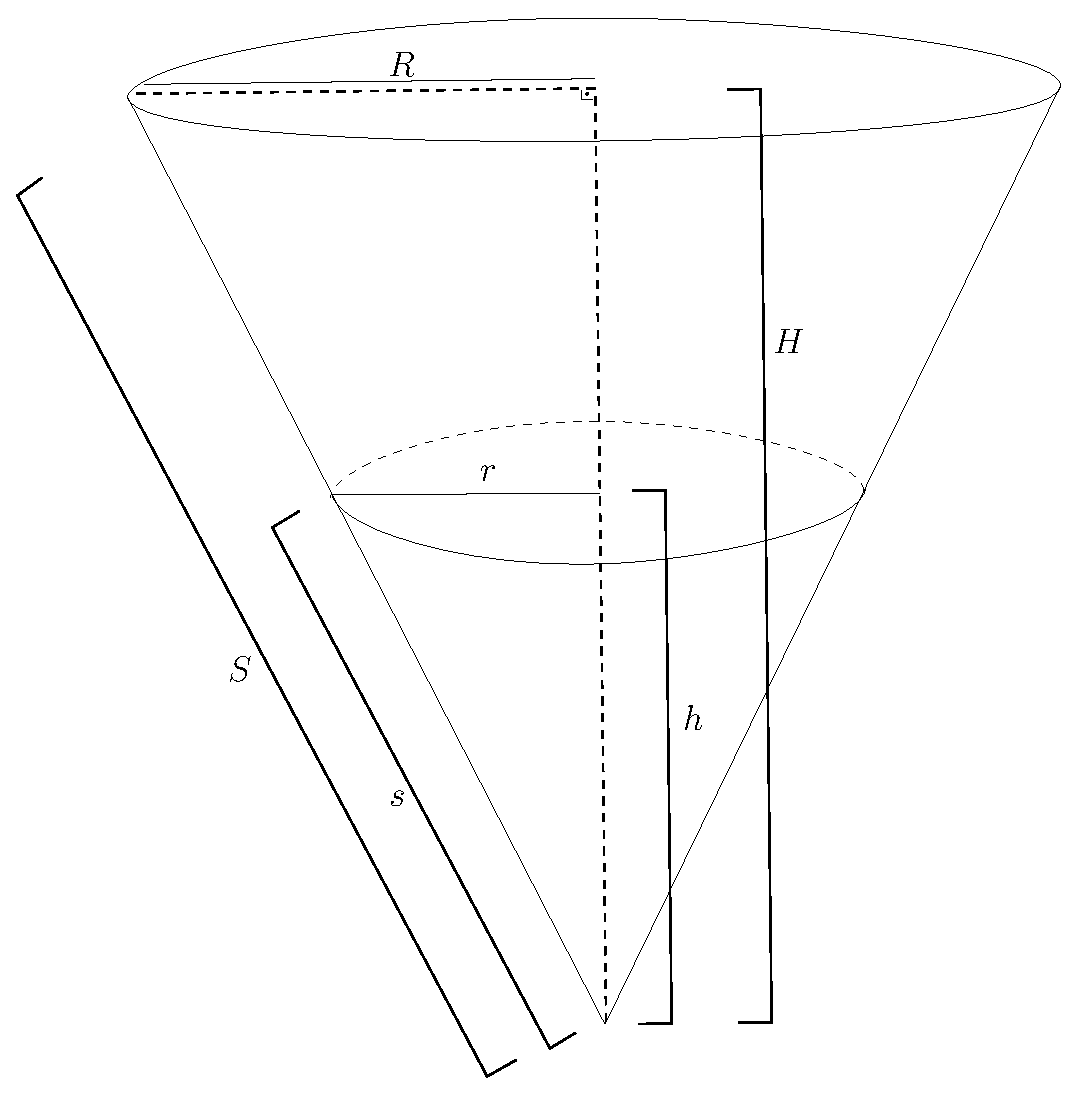
\includegraphics[scale=.5]{images/fullCone3.eps}
	\caption{Kegelstumpf und Ergänzungskegel}
	\label{fig:coneWithFrustum}
\end{figure}

\begin{figure}[!htb]
	\centering
	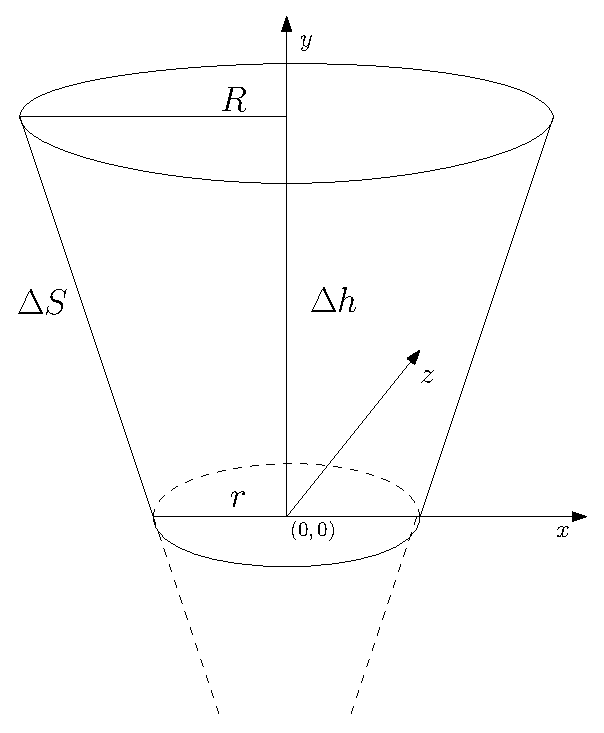
\includegraphics[scale=.7]{images/coneFrustum.eps}
	\caption{Kegelstumpf}
	\label{fig:coneFrustum}
\end{figure}

Analog zum Kreiskegel definieren wir einen Kegelstumpf durch folgende Parametrisierung: 
\begin{equation} \label{eq:paramFrustum}
\begin{aligned}
x &= (r + \frac{u}{\Delta H} (R - r))~cos \theta \\
y &= u \\
z &= (r + \frac{u}{\Delta H} (R - r))~sin \theta
\end{aligned}
\end{equation}
mit $u\in [0, \Delta H]$ und $\theta \in [0, 2\pi)$


\begin{figure}[!htb]
	\centering
	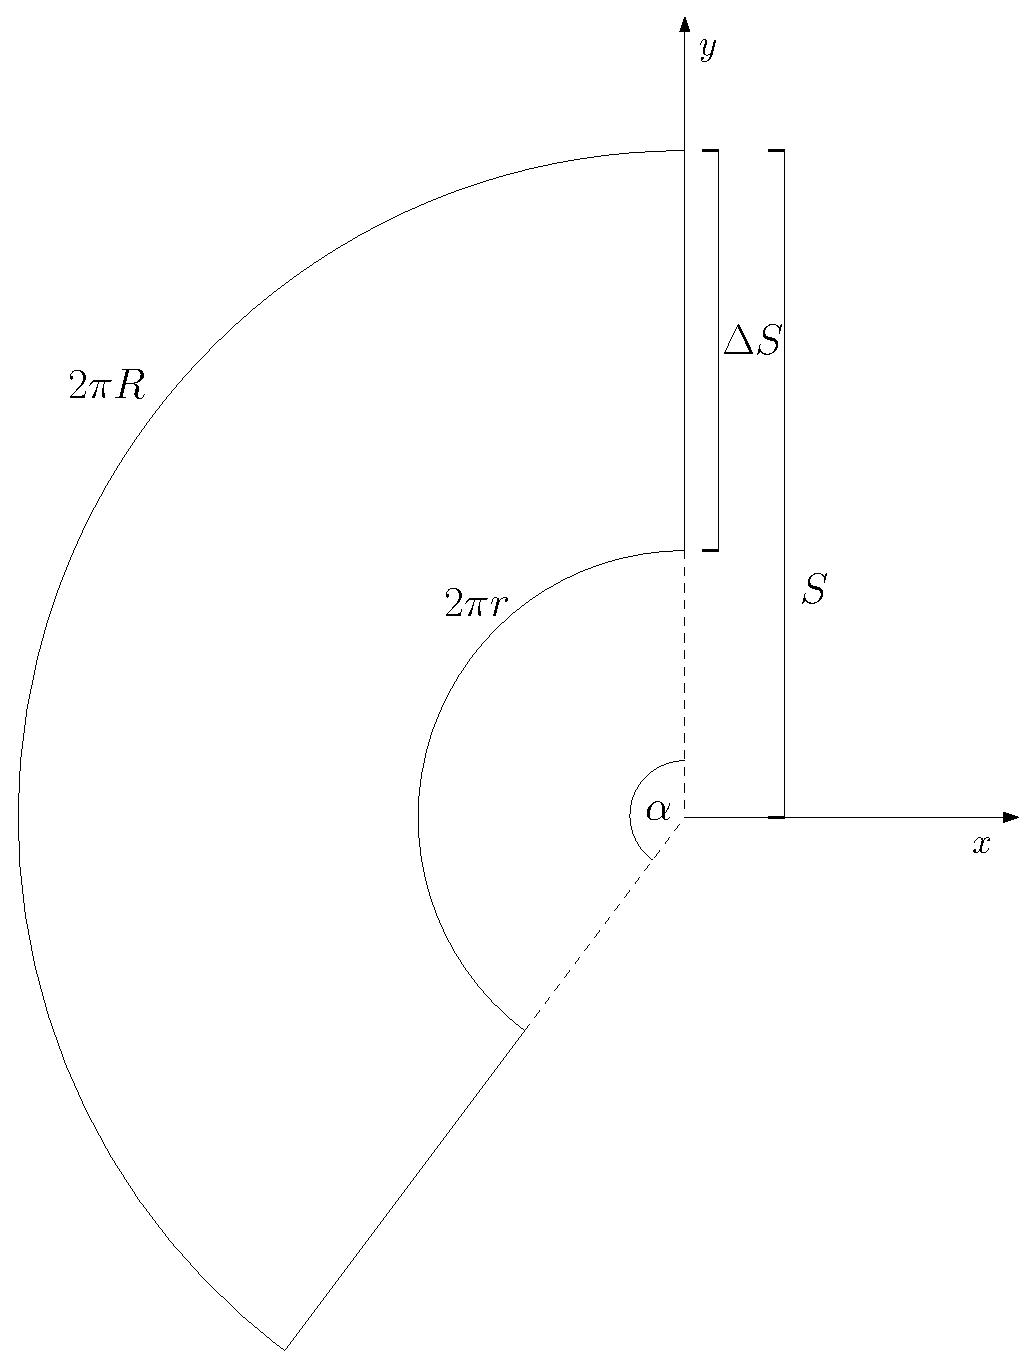
\includegraphics[scale=.4]{images/coneLateral.eps}
	\caption{Kegelmantelfläche}
	\label{fig:coneLateral}
\end{figure}

Die Mantefläche des Kegelstumpfes aus Abbildung \ref{fig:coneLateral} kann dann parametrisch beschrieben werden als:
\begin{equation} \label{eq:paramLateral}
\begin{aligned}
x &= -(s + \frac{u}{\Delta H}(S-s)) ~sin \phi \\
y &= (s + \frac{u}{\Delta H} (S-s)) ~cos \phi
\end{aligned}
\end{equation}
mit  $u\in [0, \Delta H]$ und $\phi \in [0, \alpha] \subseteq [0, 2\pi]$ mit $\alpha S = 2\pi R \implies \alpha = 2\pi\frac{R}{S}$


Ein Punkt auf der Oberfläche des Kegelstumpfs kann eindeutig einem Punkt auf der Mantelfläche (und umgekehrt) zugeordnet werden. Dazu konstruieren wir folgende Abbildung und ihr Inverses:

Sein ein Punkt $C(x,y,z)$ auf der Oberfläche des Kegelstumpfs gegeben. Wir wissen aus der parametrischen Form \ref{eq:paramFrustum}, dass $C$ die Form
\[
C(x,y,z) = (r + \frac{u}{\Delta H} (R - r))~cos \theta, u, (r + \frac{u}{\Delta H} (R - r))~sin \theta
\]  für ein $u\in [0, \Delta H]$ und $\theta \in [0, 2\pi)$ besitzt. 

Aus der $y$-Koordinate kann man als die Höhe ablesen und somit den Radius in der Mantelfläche als lineare Interpolation zwischen $s$ und $S$ bestimmen (siehe Abbildung \ref{fig:mapToLateralS}). Wir definieren uns hierfür eine Hilfsfunktion 
\begin{equation} \label{eq:Sigma}
	\Sigma(y) := s + \frac{y}{\Delta H} (S-s)
\end{equation}


\begin{figure}[!htb]
	\centering
	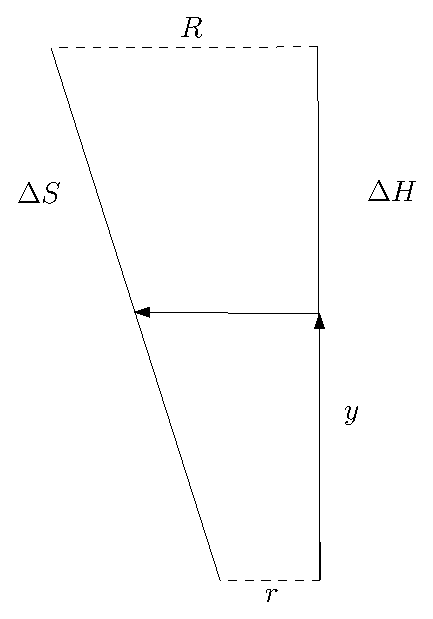
\includegraphics[scale=.7]{images/mapToLateralS.eps}
	\caption{Abbildung der Kegelstumpfhöhe auf die Seitenhöhe}
	\label{fig:mapToLateralS}
\end{figure}

Da $R, r, \Delta H$  und nun auch die Höhe bekannt sind, kann man den Winkel $\theta$ im Kegelstumpf einfach ausrechnen. Anschließend muss dieser noch mit  $\frac{R}{S}$ multipliziert werden um ihn auf $[0, \alpha]$ zu skalieren (siehe \ref{eq:paramLateral}).  Auch hierfür definieren wir eine Hilfsfunktion:
\begin{equation*}
\Phi(x,y,z) := \frac{R}{S} \atant\left(\frac{z}{r + \frac{y}{\Delta h} (R - r)}, \frac{x}{r + \frac{y}{\delta H} (R - r)}\right)
\end{equation*}

, wobei wir $\atant$ benutzen um den Winkel im richtigen Quadranten, also in $[0, 2\pi)$, bestimmen zu können. 

Mit diesen beiden Hilfsfunktionen und \ref{eq:paramLateral} ergibt sich insgesamt:
\begin{equation}
\begin{aligned}
\Psi \colon [r,R] \times [0, \Delta H] \times [r,R] &\to [s,S] \times [s,S]\\
\begin{pmatrix}
x \\ y \\ z
\end{pmatrix}  &\mapsto
\begin{pmatrix}
-\Sigma(y)\sin \Phi(x,y,z)\\
 \Sigma(y)\cos\Phi(x,y,z)
\end{pmatrix}
\end{aligned}
\end{equation}

Analog lässt die sich Umkehrabbildung konstruieren:

Sein ein Punkt $L(x,y)$ auf der Mantelfläche des Kegelstumpfs gegeben. Aus der parametrischen Form \ref{eq:paramLateral} ergibt sich

\[
L(x,y) = (-(s + \frac{u}{\Delta H}(S-s)) ~sin \phi, (s + \frac{u}{\Delta H} (S-s)) ~cos \phi)
\]

für ein passendes $u\in [0, \Delta H]$ und $\phi \in [0, \alpha] \subseteq  [0, 2\pi]$
Da $L(x,y)$ in Polarkoordinaten gegeben ist, lässt sich der Radius durch $\sqrt{x^2+y^2}$ bestimmen. Wir können den Winkel $\phi$ mit inverser Skalierung also analog durch folgende Hilfsfunktion bestimmen:

\begin{equation*}
\Theta(x,y) := \frac{S}{R} \atant\left(\frac{x}{-\sqrt{x^2+y^2}}, \frac{z}{\sqrt{x^2+y^2}}\right)
\end{equation*}

Die Höhe  im Kegel und somit der Radius lässt sich nun gewissermaßen als Umkehrabbildung zu \ref{eq:Sigma} bestimmen:
\begin{equation*}
\mathrm{H}(x,y) := \frac{\left(\sqrt{x^2+y^2}\right) - s}{S - s}\Delta H
\end{equation*}

Insgesamt ergibt sich:
\begin{equation}
\begin{aligned}
\Psi^{-1} \colon  [s,S]x[s,S] &\to [r,R] \times [0, \Delta H] \times [r,R]\\
\begin{pmatrix}
x \\ y
\end{pmatrix} &\mapsto
\begin{pmatrix}
\left( r + \frac{\mathrm{H}(x,y)}{\Delta H} (R - r)\right)\cos\left(\Theta(x,y) \right) \\
\mathrm{H}(x,y)\\
\left( r + \frac{\mathrm{H}(x,y)}{\Delta H} (R - r)\right)\sin\left(\Theta(x,y) \right)
\end{pmatrix}
\end{aligned}
\end{equation}




\todo{dieses kapitel sollte aussagekräftig sein, da projektive geometrie im titel vorkommt}
\section{Kamerakalibrierung und projektive Geometrie}
\label{s:calib}

\begin{definition}
	Kamerakalibrierung ist ein Verfahren, bei dem die interne Kamerageometrie und optischen Eigenschaften (intrinische Parameter) 
	und/oder die 3D-Position und Orientierung der Bildebene relativ zu einem Weltkoordinatensystem (extrinische Parameter) bestimmt werden \cite{Tsai1987}.
\end{definition}

\begin{figure}[!htb]
	\centering
	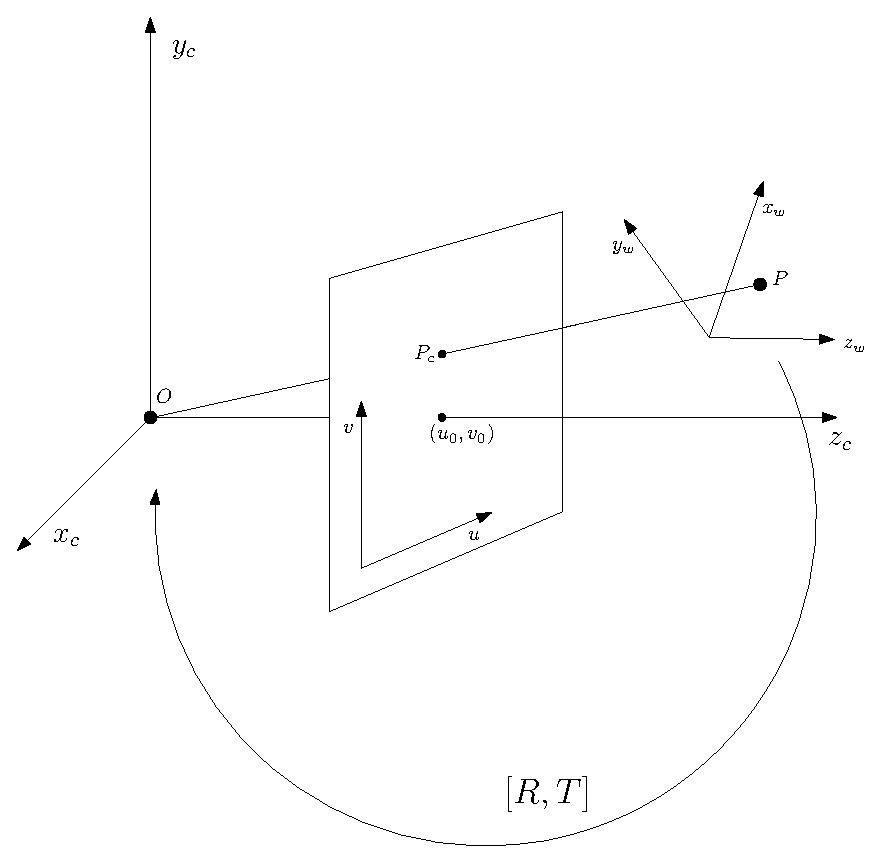
\includegraphics[scale=.8]{images/pinhole.eps}
	\caption{Projektion eines Punktes $P$ im Weltkoordinatensystem $(x_w, y_w, z_w)$ auf die Bildebene im Kamerakoordinatensystem  $(x_c, y_c, z_c)$}
	\label{fig:pinhole}
\end{figure}

Lochkamera bild, erklären warum man eine virtuelle Bildebene for die Kamera macht, damit sich das bild nicht dreht. die optischen eigenschaften ändern sich nicht.

Kamerakalibrierung wird benötigt, um eine Beziehung zwischen Punkten in 3D im Weltkoordinatensystem und den Punkten auf der Bildebene herzustellen. Genauer suchen wir eine Abbildung 

\begin{equation}
	\begin{pmatrix}
	wu \\wv \\w 
	\end{pmatrix} = 
		\begin{pmatrix}
		t_{11} & t_{12} & t_{13} & t_{14} \\
		t_{21} & t_{22} & t_{23} & t_{24} \\
		t_{31} & t_{32} & t_{33} & t_{34} 
		\end{pmatrix} 	\begin{pmatrix}
		x \\y \\z \\ 1 
		\end{pmatrix},
\end{equation}

die einen Punkt $P=(x,y,z)$ in homogenen Koordinaten $\tilde P = (x,y,z,1)$ auf einen Punkt $C = (u,v)$ auf die Bildebene abbildet.


Schritt einzeln erkklären
Zunächst wird das Weltkoordinatensystem mit einer Rotation und einer Translation in das Kamerakoordinatensystem überführt. 

Selfcalibrating vs bla bla

 erst mal außen vor. erst nach dem rest
Zu den intrinsischen Parametern gehören neben Brennweite $f$ der Kamera, die Bildmitte (auch Bildmittelpunkt) $(u_0, v_0)$, metrische Pixelgrößen $s_x$ und $s_y$, sowie Verzerrungskoeffizienten.
Mit Hilfe der intrinsischen und extrinsischen Parameter lässt sich eine 

wofür braucht man das? billige linsen, verzerrungen, 3d rekonstruktionen. abbildung von 3d auf 2d, lochkamera, intrinisch, extrinsisch
Lochkamera


Linsenverzerrungen

projektionsmatrix
(homogene Koordinaten????)
SVD, QR, LSQ?






\section{Ellipsen}
\label{s:ellipse}
\subsection{allgemein}
\label{s:ellipseGeneral}

\todo{wie schreibt man Achsen-ausgerichtet?}
\todo{wie viele punkte braucht man zum definieren von Ellipsen}
Ellipsen sind deshalb für diese Arbeit interessant, als dass sie als perspektivische Verzerrung von Kreisen entstehen. Nimmt man das Kalibrierungsmuster nicht perfekt im Lot auf, entstehen zwangsläufig Ellipsen. 

\begin{definition}[Ellipse]
	Ellipsen entstehen durch 
	Kegelschnitt und so bla bla. im weiteren bla bla meinen wir mit Hauptachsen immer die Semihauptachsen
\end{definition}

In ihrer einfachsten Form liegt die Ellipse im Zentrum des Koordinatensystems und ihre Haupt- und Nebenachse $a$ und $b$ sind Achsen-ausgerichtet, das heißt ihre Hauptachse liegt auf der $X$-Achse und ihre Nebenachse auf der $Y$-Achse. Sie kann dann in der impliziten Form

\begin{equation} \label{eq:ellipseNoRotNoTrans}
\frac{x^2}{a^2} + \frac{y^2}{b^2} = 1
\end{equation} 

beschrieben werden.

\begin{figure}[!htb]
	\centering
	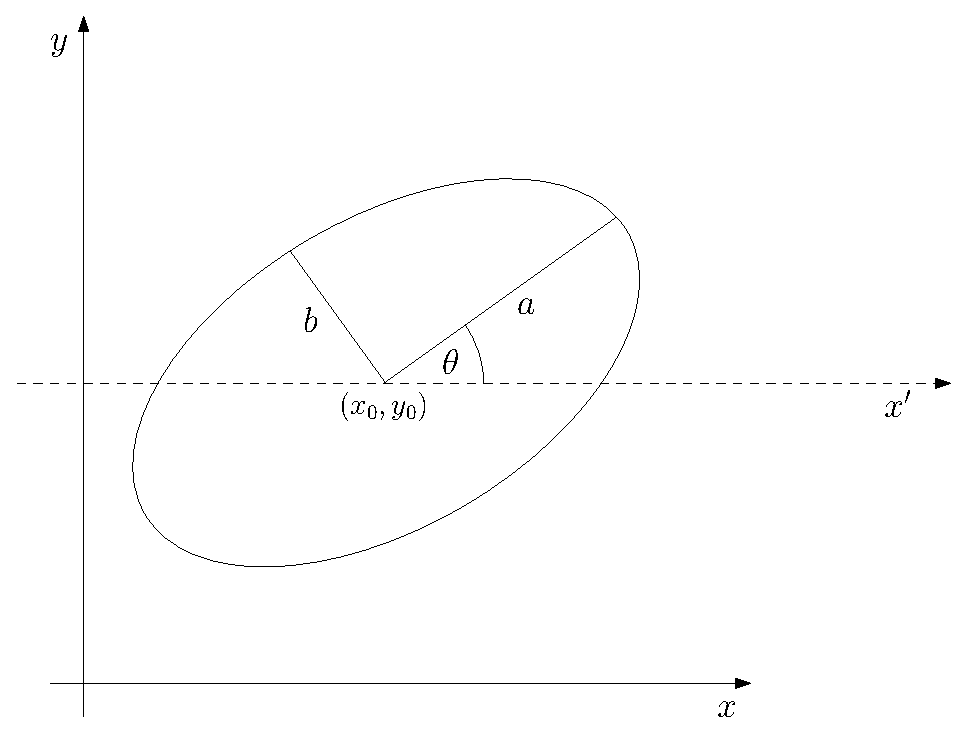
\includegraphics[scale=.7]{images/ellipse.eps}
	\caption{Ellipse mit Zentrum $(x_0, y_0)$, Hauptachse $a$, Nebenachse $b$, sowie Drehwinkel $\theta$}
	\label{fig:ellipse}
\end{figure}

Befindet sich die Ellipse nicht im Ursprung so muss eine Verschiebung beziehungsweise bei einer Rotation ein Drehwinkel (siehe Abbildung \ref{fig:ellipse}) ergänzt werden. 

\begin{equation} \label{eq:ellipseNoRotTrans}
\frac{\left(x-x_0\right)^2}{a^2} + \frac{\left(y-y_0\right)^2}{b^2} = 1
\end{equation} 

\begin{equation} \label{eq:ellipseRotTrans}
\frac{((x - x_0)\cos\theta + (y - y_0)\sin\theta)^2}{a^2} + \frac{((x - x_0)\sin\theta - (y - y_0)\cos\theta)^2}{b^2} = 1
\end{equation} 

mit Ellipsenzentrum $(x_0,y_0)\in\mathbb{R}^2$, Hauptachsen $a,b\in\mathbb{R}^+$, sowie Drehwinkel $\theta \in [0,2\pi)$ oder parametrisiert

\begin{equation} \label{eq:ellipseRotTransParam}
\begin{pmatrix}x \\ y\end{pmatrix} = \begin{pmatrix}x_0 + a\cos\phi\cos\theta - b\sin\phi\sin\theta \\ 
y_0 + a\cos\phi\sin\theta + b\sin\phi\cos\theta\end{pmatrix}
\end{equation}
mit $\phi \in [0, 2\pi)$, $x_0, y_0, a,b, \theta$ wie oben.

In ihrer allgemeinsten Form lässt sich eine Ellipse durch ein implizites Polynom zweiten Grades charakterisieren
\begin{equation} \label{eq:ellipseQuadratic}
ax^2 + by^2 + cxy + dx + ey + f = 0 \quad \text{mit}\quad c^2-4ab < 0
\end{equation} 
mit $a,b,c,d,e,f \in \mathbb{R}$. Eine Ellipse lässt sich also durch sechs Punkte eindeutig beschrieben (fünf, wenn man $f$ auf eins skaliert).


Die beiden Formen \ref{eq:ellipseRotTrans} und \ref{eq:ellipseQuadratic} sind äquivalent, falls die Ellipse nicht degeneriert ist (ohne Beweis). Da wir die Umformung von \ref{eq:ellipseRotTrans} nach \ref{eq:ellipseQuadratic} später brauchen, wird sie hier einmal exemplarisch vorgeführt. 

Zunächst einmal fällt auf, dass der gemischten Term $cxy$ genau dann null ist wenn, die Ellipse nicht rotiert wurde. Im ersten Schritt versuchen wir also die Rotation der Ellipse rückgängig zu machen, um den Rotationswinkel bestimmen zu können..

Die Gleichung \ref{eq:ellipseQuadratic} kann umgeformt werden zu:
\begin{equation*}
\begin{aligned}
\underbrace{\begin{pmatrix}x & y\end{pmatrix}}_{=:u^T}\underbrace{\begin{pmatrix}a & \frac{c}{2} \\ \frac{c}{2} & b\end{pmatrix}}_{=: M}\underbrace{\begin{pmatrix}x \\ y\end{pmatrix}}_{=u} +\begin{pmatrix}d & e\end{pmatrix}\underbrace{\begin{pmatrix}x \\ y\end{pmatrix}}_{=u}+ f = 0 \\
\Leftrightarrow u^TMu +\begin{pmatrix}d & e\end{pmatrix}u + f = 0 \\
\end{aligned}
\end{equation*} 
Der gemischte Term wird alleine durch $M = \begin{pmatrix}a & \frac{c}{2} \\ \frac{c}{2} & b\end{pmatrix}$ bestimmt. Da die Matrix $M$ symmetrisch ist, ist sie orthogonal diagonalisierbar. Des Weiteren hat $M$ zwei von null verschiedene Eigenwerte, denn 
\[
\det M = ab - \dfrac{c^2}{4}
\] ist nur dann gleich null, wenn $c^2 - 4ab = 0$, was ein Widerspruch zur Annahme in \ref{eq:ellipseQuadratic} ist. $M$ ist somit eine von null verschiedene Determinante und somit vollen Rang, hat also zwei von null verschiedene Eigenwerte. Insbesondere gibt es also zwei Eigenvektoren von $M$, die zueinander orthogonal sind.

Es gilt $M = S^TDS$, wobei $S\in\mathbb{R}^{2\times2}$ eine orthogonale Matrix mit den normierten Eigenvektoren als Zeilen und $D = \text{diag}(\lambda_1, \lambda_2)\in\mathbb{R}^{2\times2}$ eine Diagonalmatrix mit den beiden Eigenwerten von $M$ auf der Diagonalen ist. Ohne Beschränkung der Allgemeinheit gelte $\lambda_1 <= \lambda_2$, andernfalls vertausche die Eigenvektoren in $S$. 

Sei nun $v := Su$.
So gilt:

\begin{equation} \label{eq:PCARot}
\begin{aligned}
&u^T(S^TDS)u +\begin{pmatrix}d & e\end{pmatrix}\underbrace{(S^TS)}_{=\ind}u + f = 0 \\
\Leftrightarrow\quad &(Su)^TD(Su) +\begin{pmatrix}d & e\end{pmatrix}S^T(Su) + f = 0 \\
\Leftrightarrow\quad &v^{T}Dv +\begin{pmatrix}d & e\end{pmatrix}S^Tv + f = 0 
\end{aligned}
\end{equation}

Man kann leicht nachrechnen, dass der gemischte Teil somit eliminiert wurde. Durch Anwenden der Transformation $S$ wurde $u$ also in das Koordinatensystem, in dem die Ellipse Achsen-ausgerichtet ist,  transformiert.

Eine Rotationsmatrix mit Rotationswinkel $\theta$ ist definiert durch: 
\begin{equation}
\begin{aligned}
R = \begin{pmatrix}\cos\theta & -\sin\theta \\ \sin\theta & \cos\theta\end{pmatrix}
\end{aligned}
\end{equation}

Es gilt offenbar $S = R$ für ein geeignetes $\theta$, da die Eigenvektoren normiert und orthogonal zueinander sind. $\theta$ kann also einfach ausgerechnet werden, denn es gilt:

\begin{equation*}
\theta = \atant(\sin\theta, \cos\theta) = \atant(S_{2,1}, S_{1,1})
\end{equation*}

Multipliziert man nun \ref{eq:PCARot} aus ergibt sich:

\begin{equation}\label{eq:ellipseCenter}
\begin{aligned}
&\lambda_1v_1^2 + \lambda_2v_2^2 + \underbrace{\begin{pmatrix}d & e\end{pmatrix}S^T}_{=:(d', e')}v + f = 0 \\
\Leftrightarrow\quad &\lambda_1v_1^2 + \lambda_2v_2^2 + d'v_1 + e'v_2 + f = 0 \\
\Leftrightarrow\quad &(\lambda_1v_1^2 + d'v_1)+ (\lambda_2v_2^2 + e'v_2) + f = 0\\
\Leftrightarrow\quad &(\lambda_1v_1^2 + d'v_1) + (\frac{d'^2}{4\lambda_1} - \frac{d'^2}{4\lambda_1}) + (\lambda_2v_2^2 + e'v_2) + (\frac{e'^2}{4\lambda_2} - \frac{e'^2}{4\lambda_2}) + f = 0 \\
\Leftrightarrow\quad &\left[\lambda_1\left(v_1^2 + \frac{2d'}{2\lambda_1}v_1 + \frac{d'^2}{4\lambda_1^2}\right) - \frac{d'^2}{4\lambda_1}\right] +\left[\lambda_2\left(v_2^2 + \frac{2e'}{2\lambda_2}v_2 + \frac{e'^2}{4\lambda_2^2}\right) - \frac{e'^2}{4\lambda_2}\right] + f = 0 \\
\Leftrightarrow\quad &\lambda_1(v_1 + \underbrace{\frac{d'}{2\lambda_1}v_1}_{ = -x'_0})^2 +\lambda_2(v_2 + \underbrace{\frac{e'}{2\lambda_2}v_2}_{ = -y'_0})^2 - \underbrace{(\frac{d'^2}{4\lambda_1} + \frac{e'^2}{4\lambda_2} - f)}_{=:\sigma} = 0,
\end{aligned}
\end{equation}

da $\lambda_1, \lambda_2 \neq 0$. 

Das Zentrum der transformierten Ellipse kann nun aus \ref{eq:ellipseCenter} einfach abgelesen werden. Um das Zentrum der eigentlichen Ellipse zu bestimmen, muss mit der inversen Rotation $S^T$ multipliziert werden:
\begin{equation*}
(x_0, y_0)^T = S^T(x'_0, y'_0)^T
\end{equation*}

Obige Gleichung lässt sich anschließend weiter vereinfachen: 


\begin{equation} \label{eq:PCAKoeff}
\begin{aligned}
&\lambda_1(v_1 -x'_0)^2 +\lambda_2(v_2 -y'_0)^2 = \sigma \\
\Leftrightarrow\quad & \frac{\lambda_1}{\sigma}(v_1 -x'_0)^2 +\frac{\lambda_2}{\sigma}(v_2 -y'_0)^2  =1
\end{aligned}
\end{equation}

wobei $\sigma \neq 0$, wenn die Ellipse nicht zum Punkt entartet ist \cite{Lawrence1972}. Vergleicht man nun \ref{eq:PCAKoeff} mit \ref{eq:ellipseNoRotTrans} so sieht man das

\begin{equation}
\begin{aligned}
&\frac{\lambda_1}{\sigma} = \frac{1}{a^2} &\text{und}\quad &\frac{\lambda_2}{\sigma} = \frac{1}{b^2}\\
\Leftrightarrow\quad & \sqrt{\frac{\sigma}{\lambda_1}}  = a  &\text{und}\quad & \sqrt{\frac{\sigma}{\lambda_2}}  = b
\end{aligned}
\end{equation}

Es gilt wie erwartet $a \geq b$, da $\lambda_1 \leq \lambda_2$


\subsection{Abstand: Punkt zu Ellipse}
\label{sc:distPointEllipse}
Das hier beschriebene Verfahren zur Bestimmung der kürzesten euklidischen Distanz eines Punktes zu einer Ellipse stammt aus der Arbeit von David Eberly \cite{Eberly2013}.
Wir betrachten nur Ellipsen im Ursprung, die Achsen-ausgerichtet sind und darüber hinaus nur Punkte im ersten Quadranten. Ansonsten wir die Ellipse in den Ursprung verschoben und um ihren entgegengesetzten Drehwinkel rotiert. Da die Ellipse dann bezüglich der $X$- und $Y$- Achse symmetrisch ist, kann der Punkt einfach durch Spiegelung in den richtigen Quadranten transformiert werden. Der Abstand ändert sich dadurch nicht. 

Wir bezeichnen von nun an $Q = (y_0, y_1)$ als eine Punkt, dessen Distanz zur Ellipse uns interessiert und $E = (x_0, x_1)$ als denjenigen eindeutigen Punkt, welcher auf der Ellipse liegt und die kürzeste euklidische Distanz vom Punkt $Q$ hat. 

Aufgrund dieser Forderungen können wir ohne Beschränkung der Allgemeinheit folgende Aussagen treffen:
\begin{itemize}
	\item Die Ellipse kann stets durch die implizite Gleichung \[\frac{x_0^2}{a^2} + \frac{x_1^2}{b^2} = 1\] mit $a \geq b \geq 0$ beziehungsweise
	in der parametrischen Form \[\mathcal{E}(\theta) = (a\cos\phi, b\sin\phi)  \tag*{$\phi \in [0, 2\pi)$}\] beschrieben werden.
	\item Es gilt $y_0,y_1,x_0, x_1 \geq 0$
\end{itemize}

Für die quadrierte Distanz von einem beliebigen Punkt $Q$ zu einem Punkt $\mathcal{E}(\theta)$ auf der Ellipse gilt dann
\begin{equation}
	F(\theta) = \abs{\mathcal{E}(\theta) - Q}^2.
\end{equation}

Die Ableitung von $F$
\begin{equation}
F'(\theta) = 2\left(\mathcal{E}(\theta) - Q\right) \cdot \mathcal{E}'(\theta).
\end{equation}

wird null, wenn $\left(\mathcal{E}(\theta) - Q\right)$ und $ \mathcal{E}'(\theta)$ zu einander orthogonal sind. Daraus folgt, dass der Vektor von $Q$ zu $E$ senkrecht zur Ellipse stehen muss.  (siehe Abbildung \ref{fig:ellipseDist}). 


\begin{figure}[!htb]
	\centering
	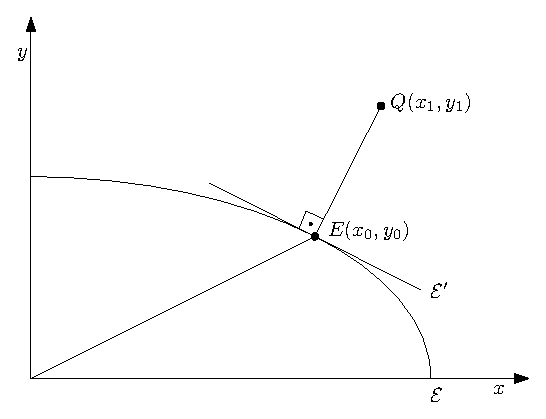
\includegraphics[scale=.9]{images/ellipseQuery.eps}
	\caption{Ellipsenausschnitt im ersten Quadranten mit Abfragepunkt $Q$ und eingezeichneter kürzester Distanz zur Ellipse}
	\label{fig:ellipseDist}
\end{figure}

Betrachten wir also die Funktion:
\begin{equation} \label{eq:ellipseDistEq}
	G(x_0,x_1) = \frac{x_0^2}{a^2} + \frac{x_1^2}{b^2} - 1.
\end{equation}
$(x_0,x_1)$ ist genau dann ein Punkt auf der Ellipse, wenn $G(x_0,x_1) = 0$. Der Gradient von $G$ in $(x_0,x_1)$ ist ein Normalenvektor auf der Ellipse, somit auch der halbe Gradient $\nabla G(x_0,x_1)/2$. Der Vektor von $E$ zu $Q$ muss dieselbe Richtung haben. Es gilt somit:

\begin{equation}
	(y_0,y_1) - (x_0, x_1) = t\frac{\nabla G(x_0,x_1)}{2} = t\left(\frac{x_0}{a^2},\frac{x_1}{b^2}\right)
\end{equation}
für ein $t\in\mathbb{R}$.

Umgestellt nach $y_0$ und $y_1$, beziehungsweise nach $x_0$ und $x_1$ ergibt sich:

\begin{equation}\label{eq:ellipseDistY}
y_0 = x_0\left(1 + \frac{t}{a^2}\right), \quad y_1 = x_1\left(1 + \frac{t}{b^2}\right)
\end{equation}

\begin{equation}\label{eq:ellipseDistX}
x_0 = \frac{a^2y_0}{t+a^2},\quad x_1 = \frac{b^2y_1}{t+b^2}
\end{equation}



Man macht nun eine Fallunterscheidung:

\begin{enumerate}
	\item Der einfachste Fall ist, wenn sich der Punkt $Q$ auf der $Y$-Achse (außer $(0,0)$) befindet, wenn also gilt $y_0 = 0, y_1 > 0$.
	Da die Hauptachse nach der $X-Achse$ ausgerichtet ist und $a >= b$ gilt, ist der Punkt auf der Ellipse mit der kürzesten Distanz zu $Q$ offenbar $E = (0, b)$ und für die Distanz gilt $d = \abs{y_1 - b}$.
	\item Als nächstes betrachten wir ein $Q$ auf der $X$-Achse (einschließlich $(0,0)$), wenn also gilt  $y_0 \geq 0, y_1 = 0$.
	
	\todo{den zweiten teil überarbeiten hier}
	Es kann gezeigt werden, dass der Punkt auf der Ellipse mit der kürzesten Distanz zu $(y_0, 0)$ für $0 < y_0 < (a^2 - b^2)/a^2$, $E = (x_0,x_1)$ ist mit 
	
	Wenn $x_1 = 0$ gilt, muss $x_0 = a$ gelten, damit $E(x_0,x_1)$ auf der Ellipse ist. Es  gilt analog zum ersten Fall $E=(a,0)$ mit $d = \abs{y_0 - a}$ 
	Einfach nur es kann gezeigt werden, dass bla? 
	
	Wenn $x_1 \neq 0$ kann gezeigt werden, dass für die Distanz gilt:
	\[
		d^2 = b^2\left(1 - \frac{y_0^2}{a^2 - b^2}\right)
	\]
	\item Der letzte Fall, den wir betrachten müssen, ist der allgemeinste Fall. Es gilt $y_0 > 0$, sowie $y_1 > 0$. Da wir uns nur im ersten Quadranten bewegen, gilt darüber hinaus $x_0, x_1 \geq 0$. Mit diesen Eigenschaften und \ref{eq:ellipseDistY} lässt sich folgende Einschränkung für $t$ herleiten:
	\begin{equation}
	\begin{aligned}
	& 0 < y_0 = x_0\left(1 + \frac{t}{a^2}\right)\\
	\Leftrightarrow\quad& -1\cdot a^2 < t.
	\end{aligned}
	\end{equation}
	Analog ergibt sich mit $y_1\colon -b^2 < t$. Da $a\geq b$ gilt, reicht es, sich nur die zweite Ungleichung anzuschauen, dass sie die erste impliziert. Setzt man nun \ref{eq:ellipseDistX} in \ref{eq:ellipseDistEq} ein, erhält man:
	
	\begin{equation}
		F(t) = \left(\frac{ay_0}{t+a^2}\right)^2 + \left(\frac{by_1}{t+b^2}\right)^2 - 1
	\end{equation}
	
	Man kann nun zeigen, dass diese Funktion auf dem gesamten Intervall $[-b^2\infty)$ monoton fällt und links gekrümmt ist. Darüber hinaus gilt:
	\[
	\lim\limits_{t \searrow -b^2}{F(t)}	= +\infty, \quad\lim\limits_{t \rightarrow \infty}{F(t)}	= 1.
	\]
	Da $F$ stetig ist, muss es also eine Nullstelle geben, die aufgrund des Monotonie- und Krümmungsverhaltens sogar eindeutig ist. Die Nullstelle lässt sich beispielsweise durch Intervallschachtelung oder Newton-Verfahren bestimmen. 
\end{enumerate}


\section{RANSAC}
\label{s:ransac}
\textit{Random Sample Consensus} (RANSAC) \cite{Fischler1981} ist ein nicht-deterministisches robustes Verfahren zur Parameterschätzung eines Modells bei einer, möglicherweise durch starke Ausreißer, gestörten Messreihe. 
Im Gegensatz zu Verfahren, wie der Methode der kleinsten Quadrate, die versuchen eine optimale Lösung für alle Messdaten zu bestimmen, nutzt RANSAC nur eine Teilmenge der Messreihe. 

\todo{Modell wortwiederholungen}
RANSAC wählt aus der Menge der Messdaten wiederholt zufällig die minimale Anzahl Messdaten aus, die nötig sind um das Modell eindeutig zu beschreiben und prüft dann, wie gut das geschätzte Modell die restlichen Messdaten beschreibt. 
Die Güte des Modells wird im Allgemeinen durch ein Distanzmaß, wie zum Beispiel der euklidische Abstand bei, charakterisiert. 
Hat ein Messdatum eine vorher definierte Maximaldistanz zum geschätzten Modell nicht überschritten, wird es ins sogenannte Consensus Set des Modells aufgenommen. 
Das Modell mit dem größten Consensus Set wird schließlich ausgewählt. 

Die Anzahl der Iterationen, die mindestens notwendig sind, um mit einer Wahrscheinlichkeit von $p \in [0,1)$, bei einem relativen Ausreißeranteil von $\epsilon \in[0,1)$ und einer Anzahl von $k$ Daten, um das Modell eindeutig zu beschreiben, lässt sich berechnen mit:

\begin{equation}
	\frac{\log{\left(1-p\right)}}{\log{\left(1-\left(1-\epsilon\right)^k\right)}}
\end{equation}




\section{Hough-Transformation für Linien}
\label{s:hough}




\section{Canny}
\label{s:canny}
Der \textit{Canny}-Algorithmus\cite{Canny1986} ist ein Verfahren zur Kantendetektion. Das 



Kantendetektion (canny sobel)

\section{Blobdetection}
\label{s:blob}
??
